% !TeX program = xelatex
\documentclass[a4paper,10pt]{article}

% ============================================================================
% សន្លឹកកិច្ចការសិស្ស ស-ខ្មៅ (Student Guided-Inquiry Worksheet - Grade 8 13.2.5 TRAP1)
% បរិបទ៖ ថ្នាក់រៀនគ្មានស្លាយ LCD – បន្ទាត់ជំនួយពីរបែបសម្រាប់ចតុកោណព្នាយ ២ ទំព័រ A4
% ============================================================================
\usepackage[a4paper, left=0.90cm, right=0.90cm, top=0.75cm, bottom=0.85cm, footskip=0.45cm]{geometry}
\usepackage{amsmath, amssymb}
\usepackage{unicode-math}
\usepackage{fontspec}
\usepackage{array, colortbl}
\usepackage[table]{xcolor}
\usepackage{enumitem}
\usepackage{pifont}
\usepackage{fancyhdr}
\usepackage{lastpage}
\usepackage{tikz}
\usepackage[most]{tcolorbox}
\usetikzlibrary{calc, arrows.meta, angles, quotes, decorations.markings, positioning, babel}

\makeatletter
\let\@expl@@@mark@update@singlecol@structures@@\relax
\makeatother

\providecommand{\NGSFindFonts}{%
  \IfFileExists{C:/Windows/Fonts/cambria.ttc}{%
    \def\NGSSysPath{C:/Windows/Fonts/}%
    \def\NGSUserPath{C:/Users/KIT/AppData/Local/Microsoft/Windows/Fonts/}%
  }{%
    \IfFileExists{./fonts/KhmerOSsiemreap.ttf}{\def\NGSSysPath{./fonts/}\def\NGSUserPath{./fonts/}}{%
    \IfFileExists{../fonts/KhmerOSsiemreap.ttf}{\def\NGSSysPath{../fonts/}\def\NGSUserPath{../fonts/}}{%
    \IfFileExists{../../fonts/KhmerOSsiemreap.ttf}{\def\NGSSysPath{../../fonts/}\def\NGSUserPath{../../fonts/}}{%
    \IfFileExists{../../../fonts/KhmerOSsiemreap.ttf}{\def\NGSSysPath{../../../fonts/}\def\NGSUserPath{../../../fonts/}}{%
    \IfFileExists{../../../../fonts/KhmerOSsiemreap.ttf}{\def\NGSSysPath{../../../../fonts/}\def\NGSUserPath{../../../../fonts/}}{%
    \IfFileExists{../../../../../fonts/KhmerOSsiemreap.ttf}{\def\NGSSysPath{../../../../../fonts/}\def\NGSUserPath{../../../../../fonts/}}{%
    \IfFileExists{../../../../../../fonts/KhmerOSsiemreap.ttf}{\def\NGSSysPath{../../../../../../fonts/}\def\NGSUserPath{../../../../../../fonts/}}{%
      \def\NGSSysPath{../../../../../../../fonts/}\def\NGSUserPath{../../../../../../../fonts/}%
    }}}}}}}%
  }%
}
\NGSFindFonts

\setmathfont[Path={\NGSSysPath}, FontIndex=1, Scale=1.02]{cambria.ttc}
\defaultfontfeatures{Ligatures=TeX}

\setmainfont[
  Path={\NGSUserPath},
  Extension=.ttf,
  Script=Khmer,
  BoldFont={KhmerOSsiemreap},
  BoldFeatures={FakeBold=1.8},
  ItalicFont={KhmerOSsiemreap},
  ItalicFeatures={FakeSlant=0.25},
  BoldItalicFont={KhmerOSsiemreap},
  BoldItalicFeatures={FakeBold=1.8, FakeSlant=0.25}
]{KhmerOSsiemreap}

\newfontfamily\muol[Path={\NGSUserPath}, Extension=.ttf, Script=Khmer]{KhmerOSmuollight}
\newfontfamily\TimesEn[Path={\NGSSysPath}, Extension=.ttf, BoldFont={timesbd}, ItalicFont={timesi}, BoldItalicFont={timesbi}]{times}

\XeTeXlinebreaklocale "km"
\XeTeXlinebreakskip = 0pt plus 1pt minus 0.1pt

\definecolor{panelgray}{gray}{0.94}
\definecolor{headgray}{gray}{0.86}
\definecolor{subgray}{gray}{0.91}

\pagestyle{fancy}
\fancyhf{}
\renewcommand{\headrulewidth}{0pt}
\fancyfoot[L]{\fontsize{8pt}{10pt}\selectfont អនុវិទ្យាល័យព្រះក្រសាំង \en{|} គណិតវិទ្យា ថ្នាក់ទី៨ \en{|} មេរៀនទី១៣ (២.៥ លក្ខណៈចតុកោណព្នាយ)}
\fancyfoot[R]{\fontsize{8.2pt}{10pt}\selectfont ទំព័រ \en{\thepage\ / \pageref{LastPage}}}

\setlength{\parindent}{0pt}
\setlength{\parskip}{0pt}
\setlength{\tabcolsep}{4pt}

\newcommand{\en}[1]{{\TimesEn #1}}
\newcommand{\enbf}[1]{{\TimesEn\textbf{#1}}}
\newcommand{\unit}[1]{\,\text{\en{#1}}}
\newcommand{\cnum}[1]{{\fontsize{10pt}{12pt}\selectfont\ding{\numexpr171+#1\relax}}}
\newcommand{\chk}{\tikz[baseline=-0.15ex]\draw[black, line width=0.8pt] (0,0) rectangle (0.25cm,0.25cm);}
\newcommand{\tri}[1]{\ensuremath{\triangle #1}}
\newcommand{\ang}[1]{\ensuremath{\angle #1}}
\newcommand{\cg}{\ensuremath{\cong}}
\newcommand{\dotline}[1]{\makebox[#1]{\dotfill}}

\newcolumntype{L}[1]{>{\raggedright\arraybackslash}p{#1}}
\newcolumntype{C}[1]{>{\centering\arraybackslash}p{#1}}

\tikzset{
  tk1/.style={postaction={decorate},decoration={markings,mark=at position 0.50 with {\draw[black, line width=0.90pt](0,-0.095)--(0,0.095);}}},
  tk2/.style={postaction={decorate},decoration={markings,
    mark=at position 0.45 with {\draw[black, line width=0.90pt](0,-0.095)--(0,0.095);},
    mark=at position 0.55 with {\draw[black, line width=0.90pt](0,-0.095)--(0,0.095);}}},
  par1/.style={postaction={decorate},decoration={markings,mark=at position 0.52 with {\draw[black, line width=0.90pt](-0.07,0.08)--(0.05,0)--(-0.07,-0.08);}}}
}

\newcommand{\secbar}[2]{%
  \vspace{3pt}
  \noindent\colorbox{headgray}{\parbox{\dimexpr\linewidth-2\fboxsep\relax}{%
    \vspace{1.5pt}{\muol\fontsize{9.5pt}{13.5pt}\selectfont #1}\hfill{\fontsize{8.5pt}{12pt}\selectfont\textbf{#2}}\vspace{1.5pt}%
  }}\par\vspace{3pt}
}

\begin{document}
\fontsize{9.5pt}{14.3pt}\selectfont

% ============================================================================
% ទំព័រទី១៖ E1 ទស្សន៍ទាយ + E2 វាស់ខ្នាតពិត 1:1 & បន្ទាត់ជំនួយពីរបែប
% ============================================================================
\begin{tcolorbox}[enhanced, sharp corners, colback=white, colframe=black, boxrule=1.0pt, top=4pt, bottom=4pt, left=6pt, right=6pt]
  \begin{center}
    {\muol\fontsize{10.5pt}{15pt}\selectfont សន្លឹកកិច្ចការសិស្ស — មេរៀនទី១៣៖ ចតុកោណ \enbf{(}២.៥ លក្ខណៈចតុកោណព្នាយ\enbf{)}}\\[2pt]
    {\footnotesize សៀវភៅសិក្សាគោលថ្នាក់ទី៨ ទំព័រ ១៨១--១៨៤ និង ១៨៦ \en{|} បំប្លែងរូបតាមបន្ទាត់ជំនួយពីរបែប (គ្មានស្លាយ \en{LCD})}
  \end{center}
  \vspace{2pt}
  \hrule height 0.5pt
  \vspace{4pt}
  ឈ្មោះសិស្សទី១៖ \dotline{3.6cm} \hspace{0.15cm} ឈ្មោះដៃគូទី២៖ \dotline{3.6cm} \hspace{0.15cm} ថ្នាក់ទី៨៖ \dotline{1.0cm} \hspace{0.15cm} ថ្ងៃទី១៨/១២/២០២៦
\end{tcolorbox}

% --- E1 Engage ---
\secbar{ផ្នែកទី១ ៖ បេសកកម្មផ្ដើមមេរៀន — កាំកណ្ដាលនៃជណ្ដើរឈើរាងចតុកោណព្នាយ \enbf{(E1 -- Engage)}}{៣ នាទី}
\begin{tcolorbox}[enhanced, sharp corners, colback=panelgray, colframe=black, boxrule=0.7pt, top=3.5pt, bottom=3.5pt, left=6pt, right=6pt]
  \textbf{ស្ថានភាពពិត៖} ជាងឈើធ្វើជណ្ដើររាងចតុកោណព្នាយ $ABCD$ ($AB\parallel DC$) មានកាំក្រោមធំ $AB = 60\unit{cm}$ និងកាំលើតូច $DC = 36\unit{cm}$ ។ គាត់ចង់កាត់កាំកណ្ដាល $EF$ ភ្ជាប់ចំណុចកណ្ដាលនៃជើងជណ្ដើរទាំងពីរ!\par\vspace{1.5pt}
  $\bullet$ \textbf{កូនជាង ក ថា៖} $EF = \frac{1}{2}(60) = 30\unit{cm}$ \hspace{0.8cm} $\bullet$ \textbf{មេជាង ខ ថា៖} $EF = \frac{60 + 36}{2} = 48\unit{cm}$\par\vspace{1.5pt}
  \textbf{ការទស្សន៍ទាយដំបូងរបស់ដៃគូអ្នក៖} \hspace{0.3cm} \chk\ កូនជាង ក ត្រូវ ($30\unit{cm}$) \hspace{0.5cm} \chk\ មេជាង ខ ត្រូវ ($48\unit{cm}$) \hspace{0.5cm} \chk\ មិនទាន់ប្រាកដ
\end{tcolorbox}

% --- E2 Explore ---
\secbar{ផ្នែកទី២ ៖ វាស់ខ្នាតពិត \enbf{1:1} និងបន្ទាត់ជំនួយពីរបែប \enbf{(E2 -- Explore)}}{១១ នាទី}
\textbf{សកម្មភាពទី១ (៤ នាទី)៖} ប្រើបន្ទាត់ក្រិត និងរ៉ាប់ព័រទ័រ វាស់ចតុកោណព្នាយសមបាតខ្នាតពិត $1:1$ ($AB=4.6\unit{cm}, DC=2.2\unit{cm}$)៖\par\vspace{3pt}
\begin{tabular}{@{}C{6.80cm} L{11.80cm}@{}}
  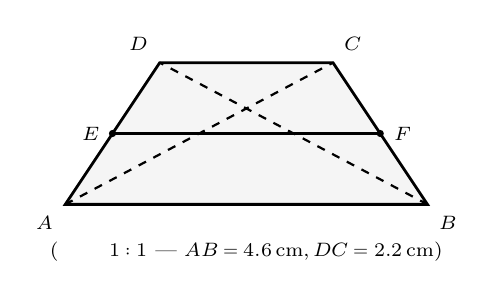
\begin{tikzpicture}[x=1cm, y=1cm, baseline={(0,1.45)}, every node/.style={font=\scriptsize, text=black}]
    % ចតុកោណព្នាយសមបាតខ្នាតពិត 1:1៖ AB = 4.6 cm, DC = 2.2 cm, h = 1.8 cm => EF = 3.4 cm គត់!
    \coordinate (A) at (0,0); \coordinate (B) at (4.6,0);
    \coordinate (D) at (1.2,1.8); \coordinate (C) at (3.4,1.8);
    \coordinate (E) at ($(A)!0.5!(D)$); \coordinate (F) at ($(B)!0.5!(C)$);
    \fill[gray!8] (A)--(B)--(C)--(D)--cycle;
    \draw[line width=1.0pt] (A)--(B)--(C)--(D)--cycle;
    \draw[line width=0.8pt, dashed] (A)--(C) (B)--(D);
    \draw[line width=1.05pt] (E)--(F);
    \fill (E) circle (1.3pt) node[left=1.5pt] {$E$};
    \fill (F) circle (1.3pt) node[right=1.5pt] {$F$};
    \node[below left=1pt] at (A) {$A$}; \node[below right=1pt] at (B) {$B$};
    \node[above right=1pt] at (C) {$C$}; \node[above left=1pt] at (D) {$D$};
    \node[anchor=north, font=\scriptsize] at (2.3,-0.35) {(ខ្នាតពិត $1:1$ — $AB=4.6\unit{cm}, DC=2.2\unit{cm}$)};
  \end{tikzpicture}
  &
  {\renewcommand{\arraystretch}{1.26}
  \begin{tabular}{|L{4.85cm}|L{6.15cm}|}
    \hline
    \rowcolor{subgray}\textbf{ធាតុដែលត្រូវវាស់} & \textbf{លទ្ធផលវាស់ និងការសង្កេត} \\
    \hline
    មុំបាត $\ang{DAB}$ និង $\ang{CBA}$ & $\ang{DAB}\approx\dotline{1.0cm}^\circ$, $\ang{CBA}\approx\dotline{1.0cm}^\circ$ (\chk\ ស្មើ) \\
    \hline
    អង្កត់ទ្រូងទាំងពីរ $AC$ និង $BD$ & $AC\approx\dotline{1.1cm}\unit{cm}$, $BD\approx\dotline{1.1cm}\unit{cm}$ (\chk\ ស្មើ) \\
    \hline
    បាតមធ្យម $EF$ (វាស់ផ្ទាល់) & $EF = \dotline{1.3cm}\unit{cm}$ \\
    \hline
    ផ្ទៀងផ្ទាត់នឹង $\dfrac{AB+DC}{2}=\dfrac{4.6+2.2}{2}$ & ស្មើនឹង $\dotline{1.3cm}\unit{cm}$ (\chk\ ត្រូវគ្នាគត់!) \\
    \hline
    ទិសដៅនៃបាតមធ្យម $EF$ ធៀបនឹងបាត & $EF \dotline{0.9cm} AB \dotline{0.9cm} DC$ (\chk\ ស្របគ្នាទាំងបី) \\
    \hline
  \end{tabular}}
\end{tabular}

\vspace{6pt}
\textbf{សកម្មភាពទី២ — បន្ទាត់ជំនួយពីរបែបស្រាយបញ្ជាក់ទ្រឹស្ដីបទទី១--៣ (៧ នាទី)៖} បំពេញចន្លោះតាមរូបសៀវភៅគោល ទំ.១៨២--១៨៣៖\par\vspace{3pt}
{\renewcommand{\arraystretch}{1.25}
\begin{tabular}{|L{9.15cm}|L{9.15cm}|}
  \hline
  \rowcolor{subgray}\textbf{ផ្នែក ក៖ ទ្រឹស្ដីបទទី១--២ — គូស $DE\parallel BC$ (ទំ.១៨២)} & \textbf{ផ្នែក ខ៖ ទ្រឹស្ដីបទទី៣ — គូស $CE$ កាត់បន្លាយ $BA$ ត្រង់ $G$ (ទំ.១៨៣)} \\
  \hline
  \begin{center}
  \vspace{-1pt}
  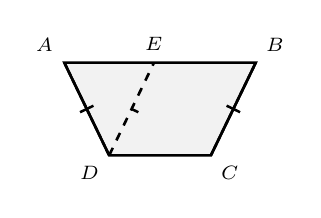
\begin{tikzpicture}[scale=0.76, every node/.style={font=\scriptsize}]
    \coordinate (D) at (0.75,0); \coordinate (C) at (2.45,0);
    \coordinate (A) at (0,1.55); \coordinate (B) at (3.20,1.55);
    \coordinate (E) at (1.50,1.55);
    \fill[gray!10] (A)--(B)--(C)--(D)--cycle;
    \draw[line width=0.95pt] (A)--(B)--(C)--(D)--cycle;
    \draw[line width=0.95pt, dashed, tk1] (D)--(E);
    \draw[line width=0.95pt, tk1] (A)--(D); \draw[line width=0.95pt, tk1] (B)--(C);
    \node[above left=0.5pt] at (A) {$A$}; \node[above=1pt] at (E) {$E$}; \node[above right=0.5pt] at (B) {$B$};
    \node[below left=0.5pt] at (D) {$D$}; \node[below right=0.5pt] at (C) {$C$};
  \end{tikzpicture}
  \vspace{-2pt}
  \end{center}
  ១. តាម $D$ គូស $DE\parallel BC$ ($E\in AB$)៖ ចតុកោណ $EBCD$ ជា \dotline{2.1cm} $\Rightarrow DE = CB$ ។\par
  ២. តែ $DA = CB$ (សមបាត) $\Rightarrow DA = \dotline{1.0cm} \Rightarrow \tri{ADE}$ សមបាត $\Rightarrow \ang{A} = \ang{AED} = \ang{\dotline{0.9cm}}$ (មុំត្រូវគ្នា)!\par
  ៣. \textbf{ទ្រឹស្ដីបទទី២៖} $\tri{ADC} \cg \tri{DBC}$ តាម (\dotline{1.3cm}: $DA=CB, \ang{D}=\ang{C}, DC$ រួម) $\Rightarrow$ អង្កត់ទ្រូង $AC = \dotline{1.1cm}$ ។
  &
  \begin{center}
  \vspace{-1pt}
  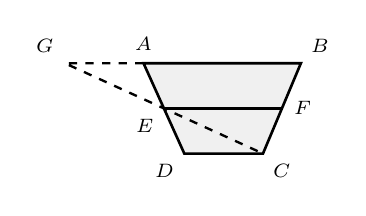
\begin{tikzpicture}[scale=0.74, every node/.style={font=\scriptsize}]
    \coordinate (G) at (0,1.55); \coordinate (A) at (1.35,1.55); \coordinate (B) at (4.05,1.55);
    \coordinate (D) at (2.05,0); \coordinate (C) at (3.40,0);
    \coordinate (E) at ($(A)!0.5!(D)$); \coordinate (F) at ($(B)!0.5!(C)$);
    \fill[gray!12] (A)--(B)--(C)--(D)--cycle;
    \draw[line width=0.95pt] (A)--(B)--(C)--(D)--cycle;
    \draw[line width=0.85pt, dashed] (A)--(G)--(E)--(C);
    \draw[line width=0.95pt] (E)--(F);
    \node[above left=0.5pt] at (G) {$G$}; \node[above=1pt] at (A) {$A$}; \node[above right=0.5pt] at (B) {$B$};
    \node[below left=0.5pt] at (D) {$D$}; \node[below right=0.5pt] at (C) {$C$};
    \node[below left=0.5pt] at (E) {$E$}; \node[right=1pt] at (F) {$F$};
  \end{tikzpicture}
  \vspace{-2pt}
  \end{center}
  ១. គូសបន្ទាត់ $CE$ កាត់បន្លាយ $BA$ ត្រង់ $G$៖ $\tri{AGE}\cg\tri{EDC}$ តាម (\dotline{1.3cm}) $\Rightarrow AG = \dotline{1.0cm}$ និង $GE = EC$ ។\par
  ២. ក្នុងត្រីកោណធំ $\tri{CGB}$៖ $E$ កណ្ដាល $GC$ និង $F$ កណ្ដាល $BC \Rightarrow EF$ ជា \dotline{2.5cm} នៃ $\tri{CGB}$!\par
  ៣. ដូច្នេះ $DC\parallel EF\parallel AB$ និង $EF = \frac{1}{2}GB = \frac{1}{2}(\dotline{1.8cm})$ ។ \\
  \hline
\end{tabular}}\par\vspace{5pt}
\begin{tcolorbox}[enhanced, sharp corners, colback=panelgray, colframe=black, boxrule=0.65pt, top=3pt, bottom=3pt, left=6pt, right=6pt]
  \textbf{សំណួរពង្រីកបន្ថែម (ទ្រឹស្ដីបទទី៤ — ចំណុចកណ្ដាលអង្កត់ទ្រូង $G, H$ ទំ.១៨៣)៖} បើ $G$ ជាចំណុចកណ្ដាល $AC$ និង $H$ ជាចំណុចកណ្ដាល $BD$ នោះ $E, G, H, F$ ស្ថិតលើបាតមធ្យមតែមួយ ($EG = \frac{1}{2}DC$ និង $HF = \frac{1}{2}DC$) ។\par\vspace{2pt}
  $\Rightarrow$ ដូច្នេះ ប្រវែងអង្កត់ភ្ជាប់ចំណុចកណ្ដាលអង្កត់ទ្រូងគឺ៖ $GH = EF - (EG + HF) = \dfrac{AB+DC}{2} - DC = \dfrac{AB - \dotline{1.1cm}}{2}$ !
\end{tcolorbox}

\newpage

% ============================================================================
% ទំព័រទី២៖ E3 ធនាគារហេតុផល ①–⑤ + E4 លំហាត់គំរូ ២ + E5 ប្រតិបត្តិ & Exit Check + កិច្ចការផ្ទះ
% ============================================================================
\secbar{ផ្នែកទី៣ ៖ សង្ខេបលក្ខណៈចតុកោណព្នាយ និងធនាគារហេតុផល \cnum{1}--\cnum{5} \enbf{(E3 -- Explain)}}{៦ នាទី}
\begin{tcolorbox}[enhanced, sharp corners, colback=white, colframe=black, boxrule=0.8pt, top=4pt, bottom=4pt, left=6pt, right=6pt]
  \cnum{1} \textbf{និយមន័យ៖} ចតុកោណព្នាយមានបាតពីរស្របគ្នា ($AB\parallel DC$); បើជ្រុងទ្រេត $AD=BC$ ហៅថា \dotline{3.2cm} ។\par\vspace{2pt}
  \cnum{2} \textbf{ទ្រឹស្ដីបទទី១៖} មុំបាតនៃចតុកោណព្នាយសមបាត \dotline{2.2cm} ($\ang{A}=\ang{B}$ និង $\ang{D}=\ang{C}$) ។\par\vspace{2pt}
  \cnum{3} \textbf{ទ្រឹស្ដីបទទី២៖} អង្កត់ទ្រូងទាំងពីរនៃចតុកោណព្នាយសមបាត \dotline{2.2cm} ($AC = BD$) ។\par\vspace{2pt}
  \cnum{4} \textbf{ទ្រឹស្ដីបទទី៣ (បាតមធ្យម)៖} បាតមធ្យមស្របនឹងបាត ហើយស្មើពាក់កណ្ដាលផលបូកបាត៖ $EF = \dfrac{\dotline{2.2cm}}{2}$ ។\par\vspace{2pt}
  \cnum{5} \textbf{ទ្រឹស្ដីបទទី៤៖} ចំណុចកណ្ដាលជ្រុងទ្រេត $E, F$ និងចំណុចកណ្ដាលអង្កត់ទ្រូង $G, H$ ស្ថិតលើ \dotline{2.5cm} ដែលស្របនឹងបាត ។
\end{tcolorbox}

% --- E4 Elaborate ---
\secbar{ផ្នែកទី៤ ៖ លំហាត់គំរូអនុវត្ត និងធនាគារហេតុផល \cnum{1}--\cnum{5} \enbf{(E4 -- Elaborate)}}{១០ នាទី}
{\renewcommand{\arraystretch}{1.24}
\begin{tabular}{|L{9.15cm}|L{9.15cm}|}
  \hline
  \rowcolor{subgray}\textbf{គំរូទី១ (លំហាត់ទី១០ក ទំ.១៨៦ — គណនាបាតតាមបាតមធ្យម)} & \textbf{គំរូទី២ (លំហាត់គំរូ ទំ.១៨៤ — ចំណុច $O, H, G$ រត់ត្រង់គ្នា)} \\
  \hline
  ក្នុងចតុកោណព្នាយ $ABCD$ ($AB\parallel DC$) មានបាតមធ្យម $XY = 12.6$ និងបាតតូច $DC = 3$ ។ គណនាប្រវែងបាតធំ $AB$ ។\par
  \begin{center}
  \vspace{-1pt}
  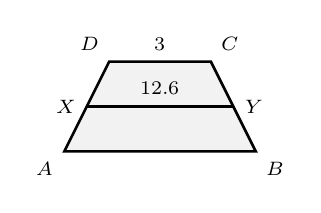
\begin{tikzpicture}[scale=0.76, every node/.style={font=\scriptsize}]
    \coordinate (D) at (0.75,1.50); \coordinate (C) at (2.45,1.50);
    \coordinate (A) at (0,0); \coordinate (B) at (3.20,0);
    \coordinate (X) at ($(A)!0.5!(D)$); \coordinate (Y) at ($(B)!0.5!(C)$);
    \fill[gray!10] (A)--(B)--(C)--(D)--cycle;
    \draw[line width=0.95pt] (A)--(B)--(C)--(D)--cycle;
    \draw[line width=0.95pt] (X)--(Y);
    \node[below left=0.5pt] at (A) {$A$}; \node[below right=0.5pt] at (B) {$B$};
    \node[above right=0.5pt] at (C) {$C$}; \node[above left=0.5pt] at (D) {$D$};
    \node[left=1pt] at (X) {$X$}; \node[right=1pt] at (Y) {$Y$};
    \node[above=0.5pt] at (1.60,1.50) {$3$}; \node[above=0.5pt] at (1.60,0.75) {$12.6$};
  \end{tikzpicture}
  \vspace{-1pt}
  \end{center}
  $\bullet$ តាមរូបមន្តបាតមធ្យម (\cnum{4})៖ $\dfrac{AB + DC}{2} = XY$\par
  $\Rightarrow AB + 3 = 2 \times \dotline{1.4cm} = \dotline{1.4cm}$\par
  $\Rightarrow AB = \dotline{1.4cm} - 3 = \dotline{1.6cm}$ ។\par\vspace{4pt}
  $\bullet$ \textbf{ផ្ទៀងផ្ទាត់៖} $\dfrac{22.2 + 3}{2} = \dotline{1.4cm}$ (ពិត!)
  &
  ចតុកោណព្នាយសមបាត $ABCD$ ($AB\parallel DC$), $G$ កណ្ដាល $AB$, $O=AD\cap BC$, $H=AC\cap BD$ ។ បង្ហាញថា $O, H, G$ ស្ថិតលើបន្ទាត់តែមួយ ។\par
  \begin{center}
  \vspace{-2pt}
  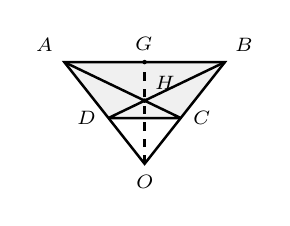
\begin{tikzpicture}[scale=0.68, every node/.style={font=\scriptsize}]
    \coordinate (O) at (1.50,0);
    \coordinate (A) at (0,1.90); \coordinate (B) at (3.00,1.90);
    \coordinate (D) at ($(O)!0.45!(A)$); \coordinate (C) at ($(O)!0.45!(B)$);
    \coordinate (G) at (1.50,1.90);
    \coordinate (H) at (intersection of A--C and B--D);
    \fill[gray!12] (A)--(B)--(C)--(D)--cycle;
    \draw[line width=0.9pt] (O)--(A)--(B)--cycle;
    \draw[line width=0.9pt] (D)--(C) (A)--(C) (B)--(D);
    \draw[line width=0.85pt, dashed] (O)--(G);
    \fill (G) circle (1.2pt) node[above=0.5pt] {$G$};
    \fill (H) circle (1.2pt) node[above right=0.5pt] {$H$};
    \node[above left=0.5pt] at (A) {$A$}; \node[above right=0.5pt] at (B) {$B$};
    \node[left=1pt] at (D) {$D$}; \node[right=1pt] at (C) {$C$};
    \node[below=0.5pt] at (O) {$O$};
  \end{tikzpicture}
  \vspace{-2pt}
  \end{center}
  $\bullet$ $\ang{OAB}=\ang{OBA}\Rightarrow \tri{OAB}$ សមបាត $\Rightarrow OG$ ជា \dotline{2.0cm} នៃ $AB$ (១)\par
  $\bullet$ $\tri{ADC}\cg\tri{BDC}\Rightarrow \ang{CAB}=\ang{DBA}\Rightarrow \tri{HAB}$ សមបាត $\Rightarrow HG$ ក៏ជា \dotline{2.0cm} នៃ $AB$ (២)\par
  $\bullet$ តាម (១) និង (២) ចំណុច $O, H, G$ ស្ថិតលើ \dotline{2.3cm} ។ \\
  \hline
\end{tabular}}\par\vspace{3pt}
$\bullet$ \textbf{ឆ្លុះបញ្ចាំង (\en{EIA})៖} បន្ទាត់ភ្ជាប់ចំណុចកណ្ដាលបាតទាំងពីរនៃចតុកោណព្នាយសមបាត ដើរតួជា \dotline{2.8cm} របស់វា!

% --- E5 Evaluate ---
\secbar{ផ្នែកទី៥ ៖ លំហាត់ប្រតិបត្តិ ផ្ទៀងផ្ទាត់ជាដៃគូ និង \enbf{Exit Check (E5 -- Evaluate)}}{១០ នាទី}
\textbf{ក. លំហាត់ប្រតិបត្តិ (លំហាត់ទី១០ខ ទំព័រ ១៨៦)៖} ក្នុងចតុកោណព្នាយ $ABCD$ ($AB\parallel DC$) មានបាតមធ្យម $XY=2x+11$, $DC=4x-7$ និង $AB=2x+1$ ។\par\vspace{3pt}
\begin{tabular}{@{}L{13.00cm} C{5.80cm}@{}}
  ១. សរសេរសមីការតាម \cnum{4}៖ $(2x+1) + (4x-7) = 2(\dotline{2.2cm})$\par\vspace{5pt}
  ២. ដោះស្រាយរក $x = \dotline{1.4cm}$ រួចគណនាប្រវែងបាតមធ្យម $XY = \dotline{1.8cm}$\par\vspace{5pt}
  ៣. \textbf{បិទបញ្ហាជណ្ដើរ E1៖} មេជាង ខ ត្រូវ ព្រោះកាំកណ្ដាល $EF = \dfrac{60+36}{2} = \dotline{1.4cm}\unit{cm}$!
  &
  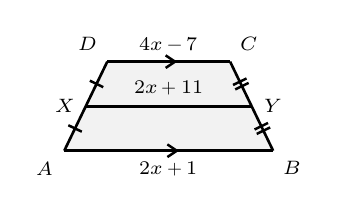
\begin{tikzpicture}[scale=0.78, baseline={(0,1.35)}, every node/.style={font=\scriptsize}]
    \coordinate (A) at (0,0); \coordinate (B) at (3.40,0);
    \coordinate (D) at (0.70,1.45); \coordinate (C) at (2.70,1.45);
    \coordinate (X) at ($(A)!0.5!(D)$); \coordinate (Y) at ($(B)!0.5!(C)$);
    \fill[gray!10] (A)--(B)--(C)--(D)--cycle;
    \draw[line width=0.95pt, par1] (D)--(C);
    \draw[line width=0.95pt, par1] (A)--(B);
    \draw[line width=0.95pt, tk1] (A)--(X); \draw[line width=0.95pt, tk1] (X)--(D);
    \draw[line width=0.95pt, tk2] (B)--(Y); \draw[line width=0.95pt, tk2] (Y)--(C);
    \draw[line width=0.95pt] (X)--(Y);
    \node[below left=0.5pt] at (A) {$A$}; \node[below right=0.5pt] at (B) {$B$};
    \node[above right=0.5pt] at (C) {$C$}; \node[above left=0.5pt] at (D) {$D$};
    \node[left=1pt] at (X) {$X$}; \node[right=1pt] at (Y) {$Y$};
    \node[above=0.5pt] at (1.70,1.45) {$4x-7$};
    \node[above=0.5pt] at (1.70,0.72) {$2x+11$};
    \node[below=0.5pt] at (1.70,0) {$2x+1$};
  \end{tikzpicture}
\end{tabular}

\vspace{4pt}
\begin{tcolorbox}[enhanced, sharp corners, colback=panelgray, colframe=black, boxrule=0.8pt, top=4pt, bottom=4pt, left=6pt, right=6pt]
  \textbf{ខ. សំណួរត្រួតពិនិត្យរហ័ស (\en{Exit Check} — គូសរង្វង់ចម្លើយត្រឹមត្រូវតែ ១)៖}\par
  ក្នុងចតុកោណព្នាយសមបាត $ABCD$ ($AB\parallel DC$) បើបាត $AB=14\unit{cm}, DC=6\unit{cm}$ និងមុំ $\ang{A}=70^\circ$ តើបាតមធ្យម $EF$ និងមុំ $\ang{D}$ ស្មើប៉ុន្មាន?\par\vspace{2pt}
  \hspace*{0.2cm}\textbf{A.} $10\unit{cm}$ និង $70^\circ$ \hspace{1.0cm} \textbf{B.} $7\unit{cm}$ និង $110^\circ$ \hspace{1.0cm} \textbf{C.} $20\unit{cm}$ និង $110^\circ$ \hspace{1.0cm} \textbf{D.} $10\unit{cm}$ និង $110^\circ$
\end{tcolorbox}

% --- Step 5 Homework ---
\secbar{ផ្នែកទី៦ ៖ កិច្ចការផ្ទះ និងបណ្ដាំផ្ញើ \enbf{(}ទំព័រ ១៨៦\enbf{)}}{ធ្វើក្នុងសៀវភៅកិច្ចការផ្ទះ}
$\bullet$ \textbf{លំហាត់ទី១១ (ទំ.១៨៦)៖} ក្នុងចតុកោណព្នាយសមបាត $ABCD$ ដែលមាន $BC\parallel AD$ និងមុំ $\ang{A} = 67^\circ$ ចូរគណនារង្វាស់មុំ $\ang{B}, \ang{C}$ និង $\ang{D}$ ។\par\vspace{2pt}
$\bullet$ \textbf{លំហាត់ទី២៖} ក្នុងចតុកោណព្នាយ $ABCD$ ($AB\parallel DC, AB=18\unit{cm}, DC=10\unit{cm}$) មាន $E, F$ កណ្ដាលជ្រុងទ្រេត និង $G, H$ កណ្ដាលអង្កត់ទ្រូង ។ គណនាប្រវែង $EF, EG, HF$ និង $GH$ រួចអានជាមុន \textbf{មេរៀនទី១៤៖ ផ្ទៃក្រឡាពហុកោណ (ទំ.១៨៧--១៩០)} ។

\end{document}
